数学における格子は、何も難しい概念ではない。
特に、2次元の場合には視覚的にも分かりやすく、例えば、2つのベクトル
\begin{align*}
\mathbf{b}_1 = \begin{pmatrix}
1\\
2
\end{pmatrix},
\mathbf{b}_2 = \begin{pmatrix}
1\\
-1
\end{pmatrix}
\end{align*}
の整数結合$x_1\mathbf{b}_1 + x_2\mathbf{b}_2$の集合である。
図示するともっと分かりやすくて、$\mathbf{b}_1 + \mathbf{b}_2$や$2\mathbf{b}_1 - \mathbf{b}_2$、$-2\mathbf{b}_1 - 3\mathbf{b}_2$などという点が格子状に配置されている(\ref{fig:lattice_example})。

\begin{figure}[htb]
\begin{center}
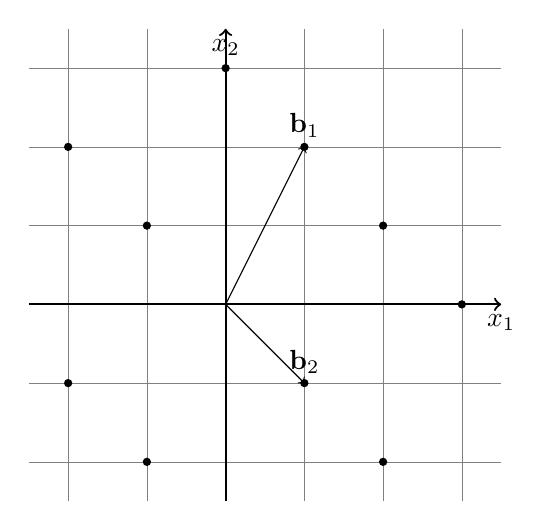
\begin{tikzpicture}
\draw [help lines] (-2.5,-2.5) grid (3.5,3.5);
\draw[thick, ->] (-2.5,0) -- (3.5,0) node [below] {$x_1$};
\draw[thick, ->] (0,-2.5) -- (0,3.5) node [below] {$x_2$};
\coordinate (O) at (0,0);
\coordinate (b1) at (1,2) node at (b1) [above] {$\mathbf{b}_1$};
\draw [->] (O) -- (b1);
\coordinate (b2) at (1,-1) node at (b2) [above] {$\mathbf{b}_2$};
\draw [->] (O) -- (b2);
\fill (b1) circle (1.5pt) (b2) circle (1.5pt) (2,1) circle (1.5pt) (0,3) circle (1.5pt) (2,-2) circle (1.5pt) (3,0) circle (1.5pt) (-1,1) circle (1.5pt) (-2,2) circle (1.5pt) (-1,-2) circle (1.5pt) (-2,-1) circle (1.5pt);
\end{tikzpicture}
\caption{$x_1\mathbf{b}_1 + x_2\mathbf{b}_2$の成す格子}
\label{fig:lattice_example}
\end{center}
\end{figure}

同じ点集合は、何も$\mathbf{b}_1,\mathbf{b}_2$でなくとも作れる。
例えば、$\mathbf{b}_1'=\begin{pmatrix}0\\3\end{pmatrix},\mathbf{b}_2' = \begin{pmatrix}1\\-1\end{pmatrix}$でも、$x_1\mathbf{b}_2' + x_2\mathbf{b}_2'$がまったく同じ点集合を成す。
実際、$\mathbf{b}_1'-\mathbf{b}_2'=\mathbf{b}_1$であることからも明らかだ。
同じようにして、どんな長いベクトルでも作れてしまうが、逆に「同じ点集合を表すベクトルの集合で、なるべく短いものは何か?」という疑問が生まれる。
それが最短ベクトル問題であり、暗号理論の分野ではしばしば暗号方式の安全性の根拠に使われる程難しい問題\Notes{SVP challenge \url{https://www.latticechallenge.org/svp-challenge/index.php}}である。
一方で応用範囲はいくつもあり、例えばRSA暗号への攻撃手法の1つにも最短ベクトル問題が関係している\Notes{RSA暗号の秘密鍵$d$が小さいと破られることが知られている。なお、\textbf{RSA暗号が破られること}と\textbf{素因数分解ができること}は等価ではないので注意。}し、もちろん本稿の主題でもある素因数分解にも使える。

改めて格子を定義しよう。

\begin{Defi}{\IND{格子}{こうし}, lattice}{lattice}
$\mathbb{R}^m$における格子とは、$\mathbb{R}^m$の$n$個の線形独立なベクトル$\mathbf{b}_1, \ldots,\mathbf{b}_n$を使って、
\begin{align*}
\Lambda = \left\{ \sum_{i=1}^n a_i \mathbf{b}_i \; : \; a_i \in\mathbb{Z} \right\}
\end{align*}
と表される集合である。
このとき、$n$を格子の\IND{階数}{かいすう}(rank)、$m$を\IND{次元}{しけん}(dimension)、$\mathbf{b}_1, \ldots,\mathbf{b}_n$を\IND{格子基底}{こうしきてい}(lattice basis)と呼ばれる。
\end{Defi}

行列では
\begin{align*}
\Lambda = \{ \mathbf{Ba} \; : \; \mathbf{a} \in \mathbb{Z}^n\}
\end{align*}
と書けるので、こちらの方が簡潔である。

LLLアルゴリズム\cite{10.1007/BF01457454}

\Algo{LLLアルゴリズム}{lll_algorithm}{}

最短ベクトル問題が解けることで、色々な問題を解くことができる。
例えば、$a_1,\ldots,a_n,N$が与えられたとき、
\begin{align*}
a_1x_1 + \cdots + a_nx_n \equiv 0 \pmod{N}
\end{align*}
を満たす$x_1,\ldots,x_n$を求める問題などは、
\begin{align*}
\mathbf{B}=
\begin{pmatrix}
1 & 0 & \cdots & 0 & a_1 \\
0 & 1 & \cdots & 0 & a_2 \\
\vdots & \vdots & \ddots & \vdots & \vdots \\
0 & 0 & \cdots & 1 & a_n \\
0 & 0 & \cdots & 0 & N
\end{pmatrix}
\end{align*}
という行列の最短ベクトル問題を解くことによって、解けるかもしれない。
方程式の解を$x_{01},\ldots,x_{0n}$としよう。
格子は$\Lambda = \{ \mathbf{Ba} \; : \; \mathbf{a} \in \mathbb{Z}^n\}$のように定義されるのだったから、
\begin{align*}
\begin{pmatrix}
1 & 0 & \cdots & 0 & a_1 \\
0 & 1 & \cdots & 0 & a_2 \\
\vdots & \vdots & \ddots & \vdots & \vdots \\
0 & 0 & \cdots & 1 & a_n \\
0 & 0 & \cdots & 0 & N
\end{pmatrix}
\begin{pmatrix}
x_{01}\\
x_{02}\\
\vdots\\
x_{0n}\\
k
\end{pmatrix}
\end{align*}
は、当然$\Lambda$に属する。
これを計算すると、$(x_{01},x_{02},\ldots,x_{0n},\sum_{i=1}^{n}a_ix_{0i} + kN)$というベクトルであって、$k=-\sum_{i=1}^{n}a_ix_{0i}/N$と置けば、$(x_{01},x_{02},\ldots,x_{0n},0)\in\Lambda$が分かる。
つまり、$(x_{01},x_{02},\ldots,x_{0n},0)$が適当に短ければ、LLLアルゴリズムで求めたベクトルが方程式の解になっている。

少し考えると、$a_1x_1 + \cdots + a_nx_n \equiv C \pmod{N}$
という形でも同じことができる。
この場合は、
\begin{align*}
\begin{pmatrix}
1 & 0 & \cdots & 0 & a_1 \\
0 & 1 & \cdots & 0 & a_2 \\
\vdots & \vdots & \ddots & \vdots & \vdots \\
0 & 0 & \cdots & 1 & a_n \\
0 & 0 & \cdots & 0 & C \\
0 & 0 & \cdots & 0 & N
\end{pmatrix}
\end{align*}
という行列を考えてやればよい。
やはり、解$x_{01},x_{02},\ldots,x_{0n}$が存在すれば、$(x_{01},x_{02},\ldots,x_{0n},-1,0)\in\Lambda$である。

他にも、多項式$f(x)$に対して、$f(x)\equiv0\pmod{N}$を満たす$x$を求める問題にも使える。
多項式の解を求めることは、整数上では簡単だが剰余環$\mathbb{Z}_N$上ではそこまで簡単な話ではない。
この問題に対するアルゴリズムとして、\IND{Coppersmithのアルゴリズム}{Coppersmithのあるこりすむ}\cite{10.1007/3-540-68339-9_14, 10.1007/3-540-68339-9_16, 10.1007/s001459900030}が有名であるが、Coppersmithオリジナルのアルゴリズムが紹介されることは少ない。
むしろその改良として発表された\IND{Howgrave-Grahamのアルゴリズム}{Howgrave-Grahamのあるこりすむ}\cite{10.1007/BFb0024458}が、Coppersmithのアルゴリズムとして扱われることもあるので、名称には注意が必要である。
なお、Coppersmithのオリジナルのアルゴリズムは上三角行列、Howgrave-Grahamのアルゴリズムは下三角行列を構成するという点でも異なっている。

さて、ある定数$X$以下の範囲にある$f(x)\equiv0\pmod{N}$の解をすべて求めたい。
方針として、$f(x)$の解と同じ解を持つ新たな多項式$g(x)$を見つける。
この$g(x)$は、仮定より解$x_0$に対して$g(x_0)\equiv0\pmod{N}$を満たすが、それよりも強く$g(x_0)=0$を満たすことを要請し、そうであるなら後は普通の多項式の解を求めるアルゴリズムを使えば済む。

そこで我々は、$f(x)\equiv0\pmod{N}$の$X$以下のすべての解$x_0$において、$g_i(x_0)\equiv0\pmod{N^m}$となるような多項式$g_i(x)$を考える(ここで、$m$はある固定された正整数である)。
このような多項式$g_i$を線形結合して作る多項式$g(x)$がもし\kenten{短い}ならば、任意の$x_0$において$g(x_0)=0$を満たす、ということが知られている。
厳密な定式化を省いて雰囲気を説明している都合上、一旦このことを納得してもらいたい。
それでも、いくつもの疑問が思い浮かぶ。

\begin{itemize}
 \item $g_i(x_0)\equiv0\pmod{N^m}$となるような多項式$g_i(x)$は簡単に見つかるのか?
 \item 最短ベクトル問題として扱うには多項式をベクトルとして扱わなければいけないが、具体的にどうすればよいのか?
\end{itemize}

1つ目については、
\begin{align*}
g_{ij}(x) = x^j N^{m-i} f^i(x)
\end{align*}
という多項式が、条件を満たす。
2つ目については、多項式$f(x)=\sum_{i=0}^k a_ix^i$に対して、ある整数$C$を使って、$(a_0, a_1C, a_2C^2,\ldots, a_kC^k)$というふうに変換してやればベクトルになるし、かつ、このベクトルのEuclid距離的に短いベクトルが、所望の多項式の\kenten{短さ}と一致する。

